\documentclass[a0paper,fontscale=0.3]{baposter}  % fontscale=0.285

\usepackage{setspace}
\usepackage{graphicx}
\usepackage{multicol}

\usepackage{tikz}
\usepackage{pgfbaselayers}
\pgfdeclarelayer{background}
\pgfdeclarelayer{foreground}
\pgfsetlayers{background,main,foreground}

%%% Color Definitions %%%%%%%%%%%%%%%%%%%%%%%%%%%%%%%%%%%%%%%%%%%%%%%%%%%%%%%%%

%\definecolor{bordercol}{RGB}{40,40,40}
%\definecolor{bordercol}{RGB}{100,0,0}
\definecolor{bordercol}{RGB}{0,0,0}
%\definecolor{headercol1}{RGB}{186,215,230}
%\definecolor{headercol2}{RGB}{80,80,80}
\definecolor{headercol1}{RGB}{153,0,0}
\definecolor{headercol2}{RGB}{153,0,0}
\definecolor{boxcolor}{RGB}{186,215,230}
\definecolor{headerfontcol}{RGB}{255,255,255}
%\definecolor{boxcolor}{RGB}{186,215,230}
\definecolor{boxcolor}{RGB}{226,200,200}
%\newcommand{\hilitetwo}[1]{{\addfontfeature{Color=FF000099}#1}}
\newcommand{\hilitetwo}[1]{{\addfontfeature{Color=99333399}#1}}
\newcommand{\hiliteone}[1]{{\addfontfeature{Color=33993399}#1}}
\newcommand{\hilitegrey}[1]{{\addfontfeature{Color=77777799}#1}}

%%% Utility functions %%%%%%%%%%%%%%%%%%%%%%%%%%%%%%%%%%%%%%%%%%%%%%%%%%%%%%%%%%

%%% Save space in lists. Use this after the opening of the list %%%%%%%%%%%%%%%%
\newcommand{\compresslist}{
        \setlength{\itemsep}{1pt}
        \setlength{\parskip}{0pt}
        \setlength{\parsep}{0pt}
}

\usepackage{polyglossia}
\setdefaultlanguage[variant=australian]{english}

\usepackage{expex}

\usepackage{fontspec}
\defaultfontfeatures{PunctuationSpace=3,Scale=MatchLowercase,Mapping=tex-text}
\newfontfeature{IPA}{+mgrk}
%\setromanfont[IPA]{FreeSerif}
%\setromanfont[IPA,Scale=0.8]{CMU Serif}
\setromanfont[IPA]{Liberation Serif}
%\setromanfont[IPA]{Times New Roman}
%\setromanfont[IPA]{NimbusRomNo9L-Regu}
%\setromanfont{Times New Roman}
%\setmonofont[IPA]{Liberation Mono}
\setmonofont[IPA]{DejaVu Sans Mono}
%\renewcommand{\sfdefault}{phv}
%\renewcommand{\rmdefault}{ptm}
%\renewcommand{\ttdefault}{pcr}
\usepackage[small,bf]{caption}
%\newfontfamily\qipa[IPA]{NimbusRomNo9L-Regu}
\newfontfamily\qipa[IPA,Scale=MatchLowercase]{FreeSerif}
\newfontfamily\qgmk[IPA,Scale=0.8]{CMU Serif}

%\newfontfamily\htwo[IPA,Scale=1.2]{FreeSans}
%\newfontfamily\htwofont[IPA,Scale=1]{CMU Sans Serif}
%\newfontfamily\htwofont[IPA,Scale=1,Color=333344FF]{CMU Sans Serif}
\newfontfamily\htwofont[IPA,Scale=1,Color=111111FF]{CMU Sans Serif}
%\newfontfamily\titlefont[IPA,Scale=0.52]{CMU Serif}
\newfontfamily\titlefont[IPA,Scale=0.7]{CMU Serif}
%\newfontfamily\titlefont[IPA,Scale=0.55]{DejaVu Serif}

%\newcommand{\htwo}[1]{::: {\htwofont #1} :::}%\hrule} %\hline\\}
%\newcommand{\htwo}[1]{{\htwofont \textbf{:::#1:::}}}%\hrule} %\hline\\}
\newcommand{\htwo}[1]{{\htwofont \textbf{\dotfill{}#1\dotfill{}}}}

%\definecolor{MyGray}{rgb}{0.96,0.97,0.98}
%\newenvironment{codebox}{%
%   \begin{lrbox}{\@tempboxa}\begin{minipage}{\columnwidth}}{\end{minipage}\end{lrbox}%
%   \colorbox{MyGray}{\usebox{\@tempboxa}}
%}
%\newcommand{\codeex}[1]{\begin{codebox}#1\end{codebox}}

%\definecolor{grey}{rgb}{0.96,0.97,0.98}
\definecolor{grey}{rgb}{0.91,0.91,0.91}
\newcommand{\codeex}[1]{
   \fbox{\colorbox{grey}{
         \begin{minipage}[t]{0.91\textwidth}
            #1
         \end{minipage}
      }
   }
}

\newcommand{\blank}[1]{\underline{\hspace{#1}}}
% FIXME: Breaks baposter
%\usepackage[novoc,fdf2alif]{arabxetex}
%\newfontfamily\uighurfont[Script=Arabic,Scale=1.5]{Lateef}
%\newfontfamily\arabicfont[Script=Arabic,Scale=1.5]{Lateef}

\usepackage{natbib}

%\makeatletter
%\renewenvironment{thebibliography}[1][]{\htwo{\bibname}}
%     {\section*{\bibname}% <-- this line was changed from \chapter* to \section*
%	  \htwo{\bibname}
%      \@mkboth{\MakeUppercase\bibname}{\MakeUppercase\bibname}%
%      \list{\@biblabel{\@arabic\c@enumiv}}%
%           {\settowidth\labelwidth{\@biblabel{#1}}%
%            \leftmargin\labelwidth
%            \advance\leftmargin\labelsep
%            \@openbib@code
%            \usecounter{enumiv}%
%            \let\p@enumiv\@empty
%            \renewcommand\theenumiv{\@arabic\c@enumiv}}%
%      \sloppy
%      \clubpenalty4000
%      \@clubpenalty \clubpenalty
%      \widowpenalty4000%
%      \sfcode`\.\@m}
%     {\def\@noitemerr
%       {\@latex@warning{Empty `thebibliography' environment}}%
%      \endlist}%}
%}
%\makeatother
%\usepackage[in]{fullpage}
\usepackage[colorlinks=true,citecolor=black,linkcolor=black,urlcolor=blue]{hyperref}

\usepackage{subfigure}
\usepackage{booktabs}

%%\bibpunct{(}{)}{;}{A}{,}{,}
%\bibdata{paper}

\newcommand{\citemultileft}[1]{(\citeauthor{#1}, \citeyear{#1}}
\newcommand{\citemultimid}[1]{\citeauthor{#1}, \citeyear{#1}}
\newcommand{\citemultiright}[1]{\citeauthor{#1}, \citeyear{#1})}
\newcommand{\citetwoyears}[2]{\citeauthor{#1} (\citeyear{#1} and \citeyear{#2})}

% for glosses
\newcommand{\eng}[1]{`{\em #1}'}
%dammit, sc doesn't seem to be working
\newcommand{\gmk}[1]{{\qgmk \textsc{#1}}}


\usepackage{enumitem}
\setlist{nolistsep,leftmargin=*}
\newenvironment{itemise}[1]{
        \begin{itemize}\setlength{\leftmargin}{-4em}\setlength{\itemsep}{-0.2em}
        \vspace{-0.5em}
        #1
}{
        \end{itemize}
        \vspace{-2pt}
}

%\newcommand{\h2}[1]{{\big



\begin{document}
	% To get it to be A0 consistently on all machines..
	%\special{papersize=1189mm,841mm}
	\special{papersize=841mm,1189mm}
	\setlength{\pdfpageheight}{\paperheight}
	\setlength{\pdfpagewidth}{\paperwidth}

%%% Setting Background Image %%%%%%%%%%%%%%%%%%%%%%%%%%%%%%%%%%%%%%%%%%%%%%%%%%
%\background{
%	
\includegraphics[width=0.99\textwidth]{flagkg2}
%}
	\background{{
%		\begin{tikzpicture}[remember picture,overlay]%
%			\draw (current page.north west)+(-4em,2em) node[anchor=north west] {
\includegraphics[width=1.1\textwidth,height=1.1\textheight]{flagkg2}};
%		\end{tikzpicture}%
%%		
\includegraphics[width=0.99\textwidth]{flagkg2}
%%			\draw (current page.north west)+(-2em,2em) node[anchor=north west] {
\includegraphics[width=0.9\textwidth]{flagkg2}};
	}}



	\begin{poster}{
			grid=false,
			%eyecatcher=false,
			borderColor=bordercol,
			headerColorOne=headercol1,
			headerColorTwo=headercol2,
			headerFontColor=headerfontcol,
			% Only simple background color used, no shading, so boxColorTwo isn't necessary
			boxColorOne=boxcolor,
			headershape=roundedright,
  headerborder=open,
  headerheight=0.08\textheight,
  %headershape=roundedright,
  %headershade=plain,
  %headerfont=\Large\textsf, %Sans Serif
			%headerfont=\Large\sf\bf,
			textborder=rectangle,
			%background=plain,
			background=user,
			headerborder=open,
			boxshade=plain,
			textborder=roundedleft,
		}{
			\hspace{-2em}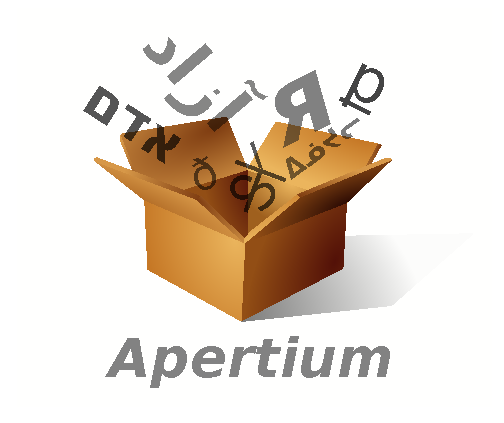
\includegraphics[height=6.5em]{apertium}
			%Eye Catcher, empty if option eyecatcher=false - unused
		}{
			{\vspace{0pt}\hspace{-2ex}
			{\titlefont \textsc{A finite-state morphological transducer for Kyrgyz}}}
		}{
			%Jonathan North Washington {\small (Indiana University, \texttt{jonwashi@indiana.edu})}, Mirlan Ipasov {\small (International Ataturk Alatoo University, \texttt{mipasov@gmail.com})}, Francis M.\ Tyers {\small (Universitat d'Alacant, \texttt{ftyers@dlsi.ua.es})}

			\vspace{-0.5em}
			\begin{center}
			{\begin{minipage}[t]{11.75em}
				\begin{spacing}{0.4}
					{Jonathan North Washington}\\
					{\footnotesize Indiana University\\\texttt{jonwashi@indiana.edu}}
				\end{spacing}
			\end{minipage}
			\begin{minipage}[t]{9.5em}
				\begin{spacing}{0.4}
					{Mirlan Ipasov}\\
					{\footnotesize International Atatürk Alatoo University\\\texttt{mipasov@gmail.com}}
				\end{spacing}
			\end{minipage}
			\begin{minipage}[t]{8em}
				\begin{spacing}{0.4}
					{Francis M.\ Tyers}\\
					{\footnotesize Universitat d'Alacant\\\texttt{ftyers@dlsi.ua.es}}
				\end{spacing}
			\end{minipage}}
			\begin{minipage}[t]{7em}
				\begin{spacing}{0.4}
					{\footnotesize Also special thanks to}\\
					{\small Tolgonay Kubatova}\\
					{\footnotesize \texttt{tolgonay@indiana.edu}}
				\end{spacing}
			\end{minipage}
			\end{center}

			%\begin{minipage}[c]{12em}
			%	\centering
			%	\begin{spacing}{0.4}
			%		Jonathan Washington\\
			%		Indiana University\\
			%		\texttt{jonwashi@indiana.edu}
			%	\end{spacing}
			%\end{minipage}
			%\begin{minipage}[c]{18em}
			%	\centering
			%	\begin{spacing}{0.4}
			%		Mirlan Ipasov\\
			%		International Ataturk Alatoo University\\
			%		\texttt{mipasov@gmail.com}
			%	\end{spacing}
			%\end{minipage}
			%\begin{minipage}[c]{10em}
			%	\centering
			%	\begin{spacing}{0.4}
			%		Francis M.\ Tyers\\
			%		Universitat d'Alacant\\
			%		\texttt{ftyers@dlsi.ua.es}
			%	\end{spacing}
			%\end{minipage}

			%Jonathan Washington, Mirlan Ipasov, Francis M.\ Tyers\\
			%Indiana University, Universitat d'Alacant, International Ataturk Alatoo University\\
			%\texttt{jonwashi@indiana.edu}, \texttt{mipasov@gmail.com}, \texttt{ftyers@dlsi.ua.es}
		}{
			%University Logo(s)
			%{\begin{minipage}{19em}
				%\hfill
				%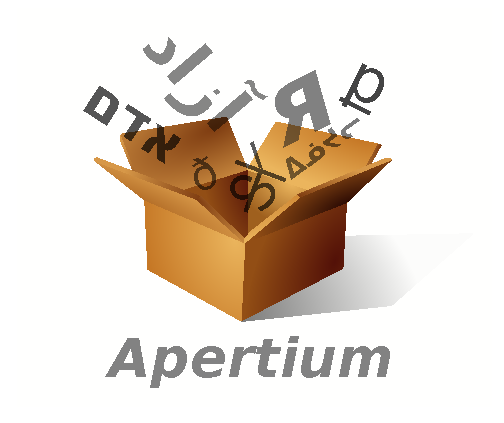
\includegraphics[height=6.5em]{apertium}
				
\includegraphics[height=6.5em]{flagkg1}
			%\end{minipage}}
		}

%		\headerbox{Overview}{name=overview,column=0,row=1}{
%			\begin{spacing}{0.8}
%This paper describes the development of a free/open-source finite-state morphological transducer for Kyrgyz. The transducer 
%has been developed for morphological generation for use within a prototype Turkish$\rightarrow$Kyrgyz machine translation system, but has also been extensively tested for analysis. The finite-state toolkit used for the work was the Helsinki Finite-State 
%Toolkit (HFST). The paper describes some issues in Kyrgyz morphology, the development of the tool, some linguistic issues encountered and how they were dealt with, and 
%which issues are left to resolve. An evaluation is presented which shows that the transducer has medium-level coverage, between 82\% and 87\% on two freely available corpora of Kyrgyz, and high precision and recall over a manually verified test set.
%			\end{spacing}\vspace{-0.25ex}
%		}
		\headerbox{Kyrgyz}{name=kyrgyz,column=0,row=0}{
			\vspace{0.5ex}
			\includegraphics[width=\textwidth]{map2}
			\vspace{-1.1em}  % -1.25em
			\begin{itemize}
				\item Turkic language (SOV, agglutinative, vowel harmony)
				\begin{itemize}
					\item Similar historically to Southern Altay
					\item Similar by convergence to Kazakh, Uzbek
				\end{itemize}
				\item Spoken in
				\begin{itemize}
					\item Kyrgyzstan, as co-official language\\
					\textit{high levels of bilingualism with Russian}
					\item China, Tajikistan, Uzbekistan
				\end{itemize}
				\item Over 3 million native speakers\\(estimate based on data from Ethnologue) %\citep{lewis2009}
				\item Our transducer based on written Kyrgyz of the former Soviet Union (literary and colloquial standards)

			\end{itemize}
		}
                \headerbox{Morphological transducers}{name=morphtrans,below=kyrgyz}{
                        \htwo{Morphological transducers}
                        \begin{itemize}
                                \item Take a surface form, and produce all valid
                                   lexical forms\\
											  e.g. `алдым'
                                \item Take a lexical form, and produce one or more
                                   valid surface forms\\
                                   e.g., \texttt{ал{\small <v><tv><ifi><p1><sg>}},
                                         \texttt{алд{\small <n><px1sg><nom>}}
                        \end{itemize}

                        \htwo{Transducers for Turkic languages}
                        \begin{itemize}
                                \item Turkish (\hiliteone{Çöltekin, 2010}; \hilitetwo{Öflazer, 1994})
                                \item Crimean Tatar (\hilitetwo{Altıntaş, 2001})
                                \item Turkmen (\hilitetwo{Tantuğ et al., 2006})
                                \item \ldots this is the first transducer for Kyrgyz
										  \item and it's \hiliteone{GPL (=free and open)}!
                        \end{itemize}

                        \htwo{Framework: HFST}
                        \begin{itemize}
                                \item Reimplementation of Xerox FST formalisms\\({\tt lexc} and {\tt twol})
                                \item Also provides a wrapper around popular free/open-source FST
                                  toolkits: SFST, OpenFST, and Foma
                        \end{itemize}

                }

%		\headerbox{Available Turkic Transducers}{name=turkictrans,below=morphtrans}{
%* Other Turkic morphological transducers\\
%		}
%		\headerbox{Framework: HFST / Apertium}{name=framework,below=turkictrans}{
%* HFST/Apertium
%		}


		\headerbox{Morphotactics}{name=lexc,below=morphtrans}{
		%\headerbox{Morphophonology}{name=morphophon,below=morphtrans}{

			\htwo{Morphological \& orthographical words}

			\begin{itemize}
				\item{} {\qipa өнүктүрөбүзбү ?} \eng{will we develop [it]?}\\
				\texttt{ өнүк{\small <v><tv><caus><aor><p1><pl>+}бы{\small <qst>}}
				\item{} {\qipa келатсаң} \eng{if you come}\\
				\texttt{кел{\tt {\small <v><iv><prt\_impf>}}+жат{\small <vaux><gna\_cnd><p2><sg>}}
			\end{itemize}

			%\htwo{Irregular negatives of finite verb forms}

			\htwo{Irregular [noun + possessive + case] forms}

			\begin{itemize}
				\item Some combinations of possessive and case morphemes are distinct (i.e., not formed simply by concatenation):

			\begin{center}
			\vspace{-0.5em}
{\small
{\qipa		
	\begin{tabular}{llllll}
		\toprule
		case & form & 1SG & 2SG & 3SP  \\
		\midrule
		nom & — & -(I)м & -(I)ң & -(S)I  \\
		acc & -NI & -(I)мдI & -(I)ңдI & -\textbf{(S)Iн}  \\
		gen & -NIн & -(I)мдIн & -(I)ңдIн & -(S)IнIн  \\
		loc & -DA & -(I)мдA & -(I)ңдA & -\textbf{(S)IндA}  \\
		abl & -DAн & -(I)мдAн, & -(I)ндAн, & -\textbf{(S)IнAн}  \\
		~   &     & -\textbf{(I)мAн} & -\textbf{(I)ңAн} \\
		dat & -GA & -\textbf{(I)мA} & -\textbf{(I)ңA} & -\textbf{(S)IнA} \\
		\bottomrule
	\end{tabular}
}}
			\end{center}

				\item Trade-off:
				\begin{itemize}
					\item morphophon.\ complicateder, morphotactics simpler
					\item underlying form used: \texttt{\{S\}\{I\}\{n\}}
					\item phonological rules delete \texttt{\{n\}}, \texttt{\{S\}} by context
				\end{itemize}
			\end{itemize}

			\htwo{Noun-noun compounds}

			\begin{itemize}
				\item one type of N-N compunds: N2 has \texttt{<px3>} and related morphology
			\end{itemize}
			\vspace{0.6ex}
			\codeex{
			{\small
			\texttt{LEXICON N-INFL-3PX-COMPOUND\\
			\vspace{-0.5ex}\%<n\%>:\%>\%\{S\%\}\%\{I\%\}\%\{n\%\} GEN-POS ;}\\
			
			\texttt{LEXICON Nouns\\
			\vspace{-0.5ex}аба\%\ ырайы:аба\%\ ырай\ N-INFL-3PX-COMPOUND ;\\\vspace{-0.5ex}\hspace{0.1pt}\hfill{}!\ "weather"\\
			\vspace{-0.5ex}чакыруу\%\ кагазы:чакыруу\%\ кагаз\ N-INFL-3PX-\\\vspace{-0.5ex}\hspace{0.1pt}\hfill{}COMPOUND ;\ !\ "invitation"}}
			}
				
			\vspace{0.5ex}
			%чакыруу кагазы
		}

					\renewcommand{\arraystretch}{0.65}
%		\headerbox{The Transducer}{name=transducer,column=0,span=2,row=1}{
%Tagset\\
%* something witty\\
%
%Things we do well\\
%* Morphophonology\\
%** vowel harmony\\
%** voicing assimilation\\
%** desonorisation\\
%* N-N compounds (чакыруу кагазы) ?
%
%
%		}

		\headerbox{Example output}{name=exout,span=2,column=1,row=0}{

		\htwo{Gloss}

		\pex[aboveexskip=0pt,belowexskip=3pt]\label{ex:sent}
			\begingl
				\gla[everygla={\qipa }]  Үстөл жана отургучтардын астын карап жатат, бирок Азамат аякта эмес. //
				\glb table and chairs' underside looking is, but Azamat there not. //
				\glft \vspace{-0.5em}\eng{[She's] looking under the tables and chairs, but Azamat isn't there.} //
			\endgl
		\xe
		
		\htwo{Output}

\noindent\texttt{\^{}\hilitetwo{Үстөл}/\hiliteone{Үстөл<n><nom>}\$\\
\^{}\hilitetwo{жана}/\hilitegrey{жан<v><iv><prc\_impf>}/\hilitegrey{жана<adv>}/\hiliteone{жана<cnjcoo>}\$\\
\^{}\hilitetwo{отургучтардын}/\hiliteone{отургуч<n><pl><gen>}\$\\
\^{}\hilitetwo{астын}/\hiliteone{аст<n><px3pl><acc>}/\hilitegrey{аст<n><px3sg><acc>}\$\\
\^{}\hilitetwo{карап}/\hilitegrey{кара<v><iv><gna\_perf>}/\hilitegrey{кара<v><iv><prc\_real>}/\hilitegrey{кара<v><tv><gna\_perf>}/\hiliteone{кара<v><tv><prc\_real>}\$\\ %¹\hfill {\textrm {\footnotesize (¹ transitive forms removed)}} \\%\footnote{tv readings removed}\\
\^{}\hilitetwo{жатат}/\hilitegrey{жат<vaux><aor><p3><pl>}/\hiliteone{жат<vaux><aor><p3><sg>}/\hilitegrey{жат<vaux><prc\_irre>}\$\hfill{}\textrm{{\footnotesize (intransitive verb forms removed)}}\\%²\\%\footnote{iv readings removed}\\
\^{}\hilitetwo{,}/\hilitegrey{,<cm>}\$\\ %\hfill {\textrm {\footnotesize (² intransitive verb forms removed)}}\\
\^{}\hilitetwo{бирок}/\hiliteone{бирок<cnjadv>}\$\\
\^{}\hilitetwo{Азамат}/\hiliteone{Азамат<np><ant><m><nom>}\$\\
\^{}\hilitetwo{аякта}/\hiliteone{ал<det><dem>+жак<n><loc>}/\hilitegrey{аяк<n><loc>}/\hilitegrey{аякта<v><tv><imp><p2><sg>}\$\\
\^{}\hilitetwo{эмес}/\hilitegrey{э<cop><neg><p3><pl>}/\hiliteone{э<cop><neg><p3><sg>}\$\\
\^{}\hilitetwo{.}/\hilitegrey{.<sent>}\$}

		\htwo{Tagset}

\vspace{-1.5em}
\setlength{\columnsep}{-1em}
\setlength{\topsep}{-\parskip}
%\spacing{0.8}
\begin{multicols}{3}
\begin{tabbing}
  \texttt{{\small <n>}}\hspace{3.0em} \=  Noun\\[-0.5ex]
  \texttt{{\small <np>}} \> Proper noun\\[-0.5ex]
  \texttt{{\small <v>}} \>  Verb\\[-0.5ex]
  \texttt{{\small <det>}} \>  Determiner\\[-0.5ex]
  \texttt{{\small <cnjcoo>}} \> Coord. conjunct.\\[-0.5ex]
  \texttt{{\small <cnjadv>}} \> Adv. conjunct.\\[-0.5ex]
  \texttt{{\small <adv>}} \> Adverb\\[-0.5ex]
  \texttt{{\small <vaux>}} \> Auxiliary verb\\[-0.5ex]
  \texttt{{\small <cop>}} \> Copula\\[-0.5ex]
  \texttt{{\small <iv>}} \> Intransitive\\[-0.5ex]
  \texttt{{\small <tv>}} \> Transitive\\[-0.5ex]
  \texttt{{\small <p2>}} \> Second person\\[-0.5ex]
  \texttt{{\small <p3>}} \> Third person\\[-0.5ex]
  \texttt{{\small <ant>}} \> Anthroponym\\[-0.5ex]
  \texttt{{\small <dem>}} \> Demonstrative\\[-0.5ex]
  \texttt{{\small <m>}} \> Masculine\\[-0.5ex]
  \texttt{{\small <sg>}} \> Singular\\[-0.5ex]
  \texttt{{\small <pl>}} \> Plural\\[-0.5ex]
  \texttt{{\small <nom>}} \> `Nominative'\\[-0.5ex]
  \texttt{{\small <gen>}} \> Genitive\\[-0.5ex]
  \texttt{{\small <acc>}} \> Accusative\\[-0.5ex]
  \texttt{{\small <loc>}} \> Locative\\[-0.5ex]
  \texttt{{\small <px3sg>}} \> 3rd person poss. (Singular)\\[-0.5ex]
  \texttt{{\small <px3pl>}} \> 3rd person poss. (Plural)\\[-0.5ex]
  \texttt{{\small <neg>}} \> Negative\\[-0.5ex]
  \texttt{{\small <aor>}} \> Aorist\\[-0.5ex]
  \texttt{{\small <imp>}} \> Imperative\\[-0.5ex]
  \texttt{{\small <gna\_perf>}} \> Verbal adverb (Perfect)\\[-0.5ex]
  \texttt{{\small <prc\_impf>}} \> Participle (Imperfect)\\[-0.5ex]
  \texttt{{\small <prc\_irre>}} \> Participle (Irrealis)\\[-0.5ex]
  \texttt{{\small <prc\_real>}} \> Participle (Realis)\\[-0.5ex]
  \texttt{{\small <cm>}} \> Comma\\
  
\end{tabbing}
\end{multicols}

		}


		\headerbox{Evaluation}{name=coverage,span=1,column=2,below=exout}{
			\htwo{8,466 total stems}

			\vspace{-1.5em}
			\setlength{\columnsep}{-1em}
			\setlength{\topsep}{-\parskip}
			\begin{multicols}{2}
			\begin{tabbing}
				Noun \hspace{3.0em} \= 4,972\\[-0.5ex]
				Verb \> 1,231 \\[-0.5ex]
				Adjective \> 944\\[-0.5ex]
				Proper noun \> 796\\[-0.5ex]
				Adverb \> 295 \\[-0.5ex]
				\\
				Numeral \> 63 \\[-0.5ex]
				Conjunction \> 58 \\[-0.5ex]
				Postposition \> 51 \\[-0.5ex]
				Pronoun \> 29\\[-0.5ex]
				Determiner \> 27\\[-0.5ex]
			\end{tabbing}
			\end{multicols}
			\vspace{-2em}

			\htwo{Test corpora}
			\begin{itemize}
				\item \textbf{Kyrgyz Wikipedia} dump dated 2011-09-23 
				\item All 2010 articles from \textbf{Radio Free Europe / Radio Liberty} (RFE/RL)'s Kyrgyz service (\texttt{azattyk.org})
				\item both split into 10 equal parts; coverage calculated over each separately; standard deviation of mean calculated
			\end{itemize}
			%both split into 10 equal parts; coverage calculated over each separately; standard deviation of the mean was calculated\\
			\htwo{Coverage measures}
			\begin{itemize}
				\item \textbf{Naïve coverage} - percentage of surface forms in a given corpus receiving ≥ 1 analysis\\(surface forms may have missing analyses)
				\item \textbf{Mean ambiguity} - average number of analyses for each surface form found in analyed corpus
			\end{itemize}
			\htwo{Coverage results (as of \texttt{r36739})}\\
%\centering
%\vspace{1pt}\hspace{2em}
			%%\begin{centering}
			%{\large
				\begin{tabular}{lrrrr}
					\toprule
					corpus           & tokens    & known       & cov. & amb.\\
					\midrule  
					Wikipedia & 329,524   & 270,668     & \hiliteone{\textbf{82.1\%}}       & \hiliteone{\textbf{2.35}}\\
 					RFE/RL & 4,112,558 & 3,614,193   & \hiliteone{\textbf{87.9\%}}      & \hiliteone{\textbf{2.43}}\\
					\bottomrule
				\end{tabular}
			%}
			%%\end{centering}
%		}

%		\headerbox{Precision \& recall}{name=precrecall,column=1,below=coverage}{

%			\htwo{Two measures}
			\htwo{Precision \& recall}
			\begin{itemize}
				\item selected 1000 surface forms at random from RFE/RL corpus,
				proof read analyses
				\item \textbf{Precision} (of a form's analyses \% correct): \hfill \hiliteone{\textbf{97.32\%}}
				\item \textbf{Recall} (percentage of analyses provided by the transducer that are correct for a form, by comparing against a gold standard): \hfill \hiliteone{\textbf{94.56\%}}
			\end{itemize}

%			\htwo{Results}
%
%			\vspace{-0.5em}
%			\begin{center}
%				\begin{tabular}{ll}
%					\toprule
%					Precision & Recall \\
%					\midrule 
%					97.32\% & 94.56\%  \\
%					\bottomrule
%				\end{tabular}
%			\end{center}
		}

		\headerbox{Morphophonology}{name=twol,column=1,below=exout}{
%			\htwo{Vowel harmony}
%			\begin{itemize}
%				\item two basic vowel archiphonemes:
%				\begin{itemize}
%					\item high vowel, \texttt{\{I\}}; [±back] and [±round] from prev.\ V\\
%		\begin{tabular}{ccccc}
%			\toprule
%			after & result & & after & result \\
%			\midrule
%			{\qipa и} & {\qipa и} & & {\qipa ы} & {\qipa ы} \\
%			{\qipa ү} & {\qipa ү} & & {\qipa у} & {\qipa у} \\
%			{\qipa е} & {\qipa и} & & {\qipa а} & {\qipa ы} \\
%			{\qipa ө} & {\qipa ү} & & {\qipa о} & {\qipa у} \\
%			\bottomrule
%		\end{tabular}
%					\item low vowel, \texttt{\{A\}}; [±back] and [±round] from prev.\ V\\
%					with one important exception: after \hilitetwo{у}\\
%		\begin{tabular}{ccccc}
%			\toprule
%			after & result & & after & result \\
%			\midrule
%			{\qipa и} & {\qipa е} & & {\qipa ы} & {\qipa а} \\
%			{\qipa ү} & {\qipa ө} & & {\qipa \hilitetwo{у}} & {\qipa \hilitetwo{а}} \\
%			{\qipa е} & {\qipa е} & & {\qipa а} & {\qipa а} \\
%			{\qipa ө} & {\qipa ө} & & {\qipa о} & {\qipa о} \\
%			\bottomrule
%		\end{tabular}
%
%
%				\end{itemize}
%				\item take backness and roundness of previous vowel\\
%				exception: 
%
%			\end{itemize}

			\htwo{Desonorisation}
\begin{itemize}
	\item {\texttt \{N\}} desonorises to д after a consonant\\
		алма-\hiliteone{\{N\}}\{I\} → алма\hiliteone{н}ы \eng{apple--\gmk{ACC}} \\
		сыр-\hiliteone{\{N\}}\{I\} → сыр\hiliteone{д}ы \eng{secret--\gmk{ACC}}
	\item {\texttt \{L\}} desonorises to д after cons.\ of sonority ≤ /l/ \\
		сыр-\hiliteone{\{L\}}\{A\}р → сыр\hiliteone{л}ар \eng{secret--\gmk{PL}} \\
		кыз-\hiliteone{\{L\}}\{A\}р → кыз\hiliteone{д}ар \eng{girl--\gmk{PL}} \\
\end{itemize}

	\vspace{-0.5ex}
\codeex{
			\texttt{"L Desonorisation"\\
			\%\{L\%\}:д <=> :VoicedLowSonCns \%>:\ \blank{1em} ;}\\
			
			\texttt{"N Desonorisation"\\
			\%\{N\%\}:д <=> :VoicedCns \%>:\ \blank{1em} ;}
}

			\htwo{Lenition}
\begin{itemize}
	\item Turn {\texttt \{y\}} into a harmonised high vowel when a vowel doesn't follow the following consonant:\\
	мур\{у\}н → мурун \eng{nose}\\
	мур\{у\}н+\{I\}м → мурдум \eng{my nose}\\
\end{itemize}
	\vspace{-0.5ex}
\codeex{
{\small \texttt{\%\{y\%\}:Vy <=> [ :LastVowel :Cns* :Cns ]/[:0] \blank{1em}\\
	\vspace{-0.5ex}\hspace{1pt}\hfill{} [ :Cns [ .\#.\ | :Cns ] ]/[ :0 | \%>:]\ ;\\
  \vspace{-0.5ex}\hspace{1ex}where  Vy  in  (  и  ү  и  и  ү  ы  ы  у  у  ы  у  у )\\
  \vspace{-0.5ex}LastVowel  in  (  и  ү  е  э  ө  я  а  ё  о  ы  ю  у )\\
  \vspace{-0.5ex}\hspace{12ex}         matched ;}}
}

			%\htwo{Nouns ending in /рн/}

			\htwo{й+vowel letters}
			\begin{itemize}
				\item{} [ а о у ] become [ я ё ю ] after й and й deletes
				\item й incorporated into the context of many rules
				\item + separate rules to change the characters
				\item + a rule to delete the original й\\
			\end{itemize}
	\vspace{-1ex}

				\codeex{
					\texttt{"Deletion of й before yoticised vowels"\\
					й:0 <=> \blank{1em} [ :YotVow ]/[ :0 | \%>:\ ]\ ;}
				}
		}

		\headerbox{Future Work}{name=nedostatki,column=2,below=coverage}{
			\begin{itemize}
				\item case changes for words with one root\\
					\hiliteone{Ф}инландия \eng{Finland}, \hiliteone{ф}инландиялык \eng{Finnish}
				\item phonol.\ (vowel harmony, desonorisation) with abbrevs.\\
					АКШ [акышы] \eng{USA} → АКШ\hiliteone{н}ын / *АКШ\hiliteone{т}ын
				\item vowel harmony with numbers\\
					{\qipa 100 [жүз] → 100дүн [жүздүн] / *100нын}
				\item compound verbs (esp.\ ones with changeable parts)
				\item gerunds with mono-syllabic V-final verbs\\
					{\qipa иште- \eng{work} → иштеш / иштөө \eng{working}}\\
					{\qipa же- \eng{eat} → жеш / *жөө \eng{eating}}
				\item Disambiguation
				\item More stems!
				\item Machine translation between Turkic languages
			\end{itemize}
		}

		\headerbox{Further information}{name=getting,column=1,below=twol}{
			\begin{itemize}
				\item The transducer is available from apertium's svn repo\.:\\
				info at {\small \url{http://wiki.apertium.org/wiki/apertium-kir}}

				\item Turkic RBMT mailing list (>25 subscribers):\\
				\texttt{apertium-turkic@lists.sourceforge.net}\\
				\vspace{-0.5ex}Feel free to post in any language!\\\vspace{-2.5ex}
				\item See our paper in the LREC 2012 proceedings
				\item And feel free to contact the authors any time!
			\end{itemize}
			\vspace{2.8ex}
		}


%		\headerbox{References}{name=references,column=2,below=nedostatki}{
%			%\begin{thebibliography}{1}\itemsep=-0.01em
%			\setlength{\baselineskip}{0.4em}
%		}


	\end{poster}
\end{document}
